\chapter{Software as a Service}

\section{Cloud Computing}
La differenza tra il possedere e l'utilizzare. E' questo l'aspetto cruciale del cambiamento apportato dal cloud computing rispetto al software tradizionale. Le risorse, che siano esse stesse archiviazione, elaborazione o qualsivoglia risorsa informatica, non sono mai ad hoc per un singolo utente, ma vengono assegnate on demand ai singoli utenti e appartengono ad un insieme condiviso da tutti gli altri utenti del prodotto utenti. Attraverso internet ogni utente può accedere a queste risorse in qualsiasi momento. Tali risorse vengono opportunamente allocate all'utente in maniera dinamica e completamente automatizzata. L'utente può utilizzare così anche software non installati sul proprio computer o usufruire di una memoria di massa accessibile da parte sua da qualsiasi dispositivo.
\paragraph{}
L'esperienza utente che si vuole fornire però è quella di un utilizzo esclusivo della risorsa, come nei software tradizionali, quando in realtà la risorsa viene solo sapientemente distribuita tra gli utenti. Ciò fa si che, potenzialmente, un singolo utente possa acquisire risorse notevolmente maggiori nel caso medio
\begin{figure}
	\centering
	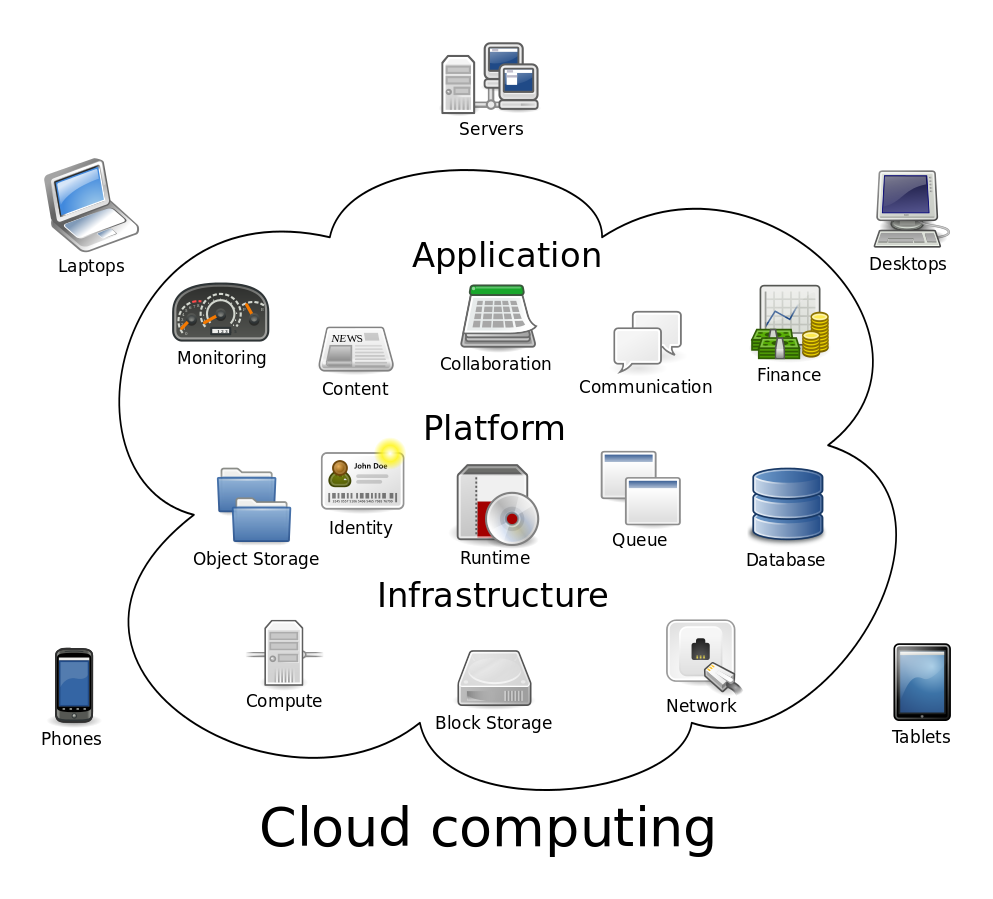
\includegraphics[width=0.7\linewidth]{capitoli/imgs/CloudComputing}
	\caption{Diagramma logico di una rete Cloud Computing}
	\label{fig:cloudcomputing}
\end{figure}
\subsection{Vantaggi del Cloud Computing}
\begin{itemize}
	\item Costo: \\
	Con l'avvento del cloud tutta la gestione dell'infrastruttura sottostante il software diviene a carico del provider. Vengono eliminate spese per la gestione dei data center locali. Facendo riferimento alla versione SaaS di BigFix ad esempio, il cliente viene sollevando dal pesante onere di utilizzare server locali e gestirne le relative connessioni. Il provider detiene tutto l'hardware di cui il cliente ha bisogno.
	
	\item Velocità: \\
	Anche quì ci risulta molto utile prendere ad esempio la suite di BigFix. quando un nuovo cliente acquista il prodotto nella sua versione on-premises, un'incaricato di IBM si reca presso il cliente e lì inizia un lungo processo di installazione della suite che può impiegare diverse ore. nella scenario SaaS il cambiamento è radicale. E' sufficente che il cliente compili una form online, dopo alcuni minuti poi riceve una mail con il link per accedere al servizio.
	
	\item Scalabilità \\
	
\end{itemize}
\subsection{Svantaggi del Cloud Computing}
https://www.bucap.it/news/approfondimenti-tematici/prodotti/significato-software-on-premise-vantaggi.htm